\documentclass{beamer}
\usepackage{amsmath}
\usepackage[english]{babel} %set language; note: after changing this, you need to delete all auxiliary files to recompile
\usepackage[utf8]{inputenc} %define file encoding; latin1 is the other often used option
\usepackage{csquotes} % provides context sensitive quotation facilities
\usepackage{graphicx} %allows for inserting figures
\usepackage{booktabs} % for table formatting without vertical lines
\usepackage{textcomp} % allow for example using the Euro sign with \texteuro
\usepackage{stackengine}
\usepackage{wasysym}
\usepackage{tikzsymbols}
\usepackage{textcomp}
\newcommand{\bubblethis}[2]{
        \tikz[remember picture,baseline]{\node[anchor=base,inner sep=0,outer sep=0]%
        (#1) {\underline{#1}};\node[overlay,cloud callout,callout relative pointer={(0.2cm,-0.7cm)},%
        aspect=2.5,fill=yellow!90] at ($(#1.north)+(-0.5cm,1.6cm)$) {#2};}%
    }%
\tikzset{face/.style={shape=circle,minimum size=4ex,shading=radial,outer sep=0pt,
        inner color=white!50!yellow,outer color= yellow!70!orange}}
%% Some commands to make the code easier
\newcommand{\emoticon}[1][]{%
  \node[face,#1] (emoticon) {};
  %% The eyes are fixed.
  \draw[fill=white] (-1ex,0ex) ..controls (-0.5ex,0.2ex)and(0.5ex,0.2ex)..
        (1ex,0.0ex) ..controls ( 1.5ex,1.5ex)and( 0.2ex,1.7ex)..
        (0ex,0.4ex) ..controls (-0.2ex,1.7ex)and(-1.5ex,1.5ex)..
        (-1ex,0ex)--cycle;}
\newcommand{\pupils}{
  %% standard pupils
  \fill[shift={(0.5ex,0.5ex)},rotate=80] 
       (0,0) ellipse (0.3ex and 0.15ex);
  \fill[shift={(-0.5ex,0.5ex)},rotate=100] 
       (0,0) ellipse (0.3ex and 0.15ex);}

\newcommand{\emoticonname}[1]{
  \node[below=1ex of emoticon,font=\footnotesize,
        minimum width=4cm]{#1};}
\usepackage{scalerel}
\usetikzlibrary{positioning}
\usepackage{xcolor,amssymb}
\newcommand\dangersignb[1][2ex]{%
  \scaleto{\stackengine{0.3pt}{\scalebox{1.1}[.9]{%
  \color{red}$\blacktriangle$}}{\tiny\bfseries !}{O}{c}{F}{F}{L}}{#1}%
}
\newcommand\dangersignw[1][2ex]{%
  \scaleto{\stackengine{0.3pt}{\scalebox{1.1}[.9]{%
  \color{red}$\blacktriangle$}}{\color{white}\tiny\bfseries !}{O}{c}{F}{F}{L}}{#1}%
}
\usepackage{fontawesome} % Social Icons
\usepackage{epstopdf} % allow embedding eps-figures
\usepackage{tikz} % allows drawing figures
\usepackage{amsmath,amssymb,amsthm} %advanced math facilities
\usepackage{lmodern} %uses font that support italic and bold at the same time
\usepackage{tikz}
\usepackage{tcolorbox}

\usefonttheme[onlymath]{serif} %set math font to serif ones

\definecolor{beamerblue}{rgb}{0.2,0.2,0.7} %define beamerblue color for later use

%%% defines highlight command to set text blue
\newcommand{\highlight}[1]{{\color{blue}{#1}}}


%%%%%%% commands defining backup slides so that frame numbering is correct

\newcommand{\backupbegin}{
   \newcounter{framenumberappendix}
   \setcounter{framenumberappendix}{\value{framenumber}}
}
\newcommand{\backupend}{
   \addtocounter{framenumberappendix}{-\value{framenumber}}
   \addtocounter{framenumber}{\value{framenumberappendix}}
}

%%%% end of defining backup slides

%Specify figure caption, see also http://tex.stackexchange.com/questions/155738/caption-package-not-working-with-beamer
\setbeamertemplate{caption}{\insertcaption} %redefines caption to remove label "Figure".
%\setbeamerfont{caption}{size=\scriptsize,shape=\itshape,series=\bfseries} %sets figure  caption bold and italic and makes it smaller


\usetheme{Boadilla}

% --------------------
% Overall information
% --------------------
\title[Economía I]{Economía I \vspace{4mm}
\\ Magistral 27: Politica fiscal}
\date{}
\author[Riottini]{Riottini Franco}
\vspace{0.4cm}
\institute[]{Universidad de San Andrés} 


\begin{document}

\begin{frame}
\titlepage
\centering

\includegraphics[scale=0.2]{../Figures/logoUDESA.jpg} 
\end{frame}

\begin{frame}{¿Cómo funciona la política fiscal?}
    \begin{itemize}
        \item El análisis de la política fiscal es mucho más complejo por una serie de motivos:
        \begin{itemize}
            \item La política fiscal expansiva genera aumentos de la demanda agregada 
            \item Pero la política fiscal requiere financiamiento
            \begin{itemize}
                \item Necesitamos entender cómo puede financiar el Gobierno para hacer uso de este instrumento
            \end{itemize}
            \item Hay efectos expulsión (“crowding out”) vía la tasa de interés (que no aparecían con la política monetaria)
        \end{itemize}
        \item La combinación de estos tres factores nos dará el efecto neto de la política fiscal sobre la demanda agregada
    \end{itemize}
\end{frame}

\begin{frame}{¿Cómo puede financiar el gasto un gobierno?}
    \begin{itemize}
        \item Existen tres mecanismos básicos para financiar la política fiscal:
        \begin{itemize}
            \item Emisión monetaria $\Rightarrow$ El fisco le pide dinero al Banco Central $\rightarrow$ Idéntico a lo que vimos en política monetaria.
            \item Aumentar los impuestos 
            \item Pedir deuda
        \end{itemize}
        \item Cada uno de estos implicará distintos mecanismos sobre la demanda agregada
    \end{itemize}
\end{frame}

\begin{frame}{El efecto “financiamiento” sobre el consumo: impuestos}
    \begin{itemize}
        \item Si aumenta el gasto público financiado enteramente con impuestos: ¿cuánto cae el consumo privado?
        \begin{itemize}
            \item Recuerden la discusión sobre suavización del consumo: los individuos quieren consumir todos los períodos \textit{parecido}
            \item Cae el consumo que esos impuestos desplazan
            \item Si los impuestos son permanentes la caída del consumo debiera ser el 100\% del aumento de los impuestos
            \item La caída del consumo es menor si se piensa que es transitorio y podría aumentar el producto en le corto plazo
            \item El efecto de la política fiscal se modera sustancialmente cuando se tiene en cuenta el financiamiento
        \end{itemize}
        \item ¿Cuándo tiene, entonces, la política fiscal un efecto sobre la demanda agregada?
        \begin{itemize}
            \item Cuando no hay una reducción equivalente del consumo privado $\rightarrow$ más dificil de lo que parece
        \end{itemize}
    \end{itemize}
\end{frame}

\begin{frame}{Expansión fiscal c/impuestos permanentes (clásico)}
    \begin{center}
        \begin{figure}[H]
        \renewcommand{\figurename}{Figure}
        \begin{center}
        \begin{minipage}[b]{0.45\textwidth}
        \begin{center}
        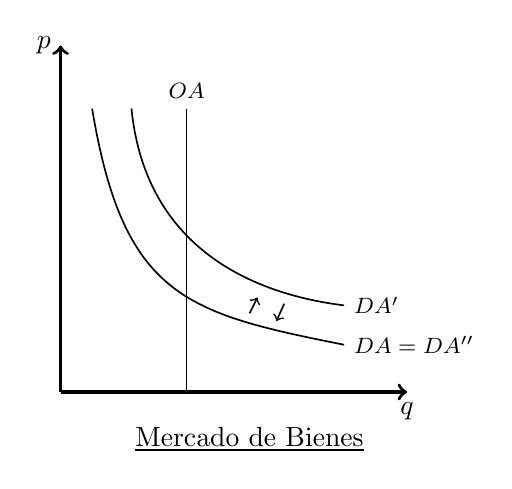
\begin{tikzpicture}[scale=0.4]
        \draw[very thick,<-] (0,11)--(0,0);
        \draw[very thick,->] (0,0)--(11,0) node[below]{$q$};
        \node[left] at (0,11) {$p$};
        \node[] at(6,-1.5) {\underline{Mercado de Bienes}};
        \draw[semithick] (1,9).. controls (2,3) and (4, 2.5) .. (9, 1.5) node [right]{\footnotesize $DA=DA''$};
        \draw[semithick] (2.25,9).. controls (2.75,4) and (7, 3) .. (9, 2.75) node [right]{\footnotesize $DA'$};
        \draw[semithick](4, 0)--(4, 9) node [above]{\footnotesize $OA$};
        \draw[semithick, ->] (6,2.5)--(6.25,3);
        \draw[semithick, <-] (6.85,2.25)--(7.1,2.8);
        \end{tikzpicture}
        \end{center}
        \end{minipage}
        \begin{minipage}[b]{0.45\textwidth}
        \begin{center}
        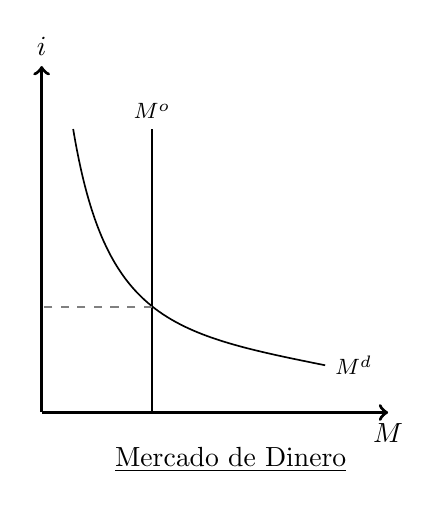
\begin{tikzpicture}[scale=0.4]
        \draw[very thick,<-] (0,11) node[above]{$i$}--(0,0);
        \draw[very thick,->] (0,0)--(11,0) node[below]{$M$};
        \node[right] at (0,11) {};
        \node[] at(6,-1.5) {\underline{Mercado de Dinero}};
        \draw[semithick] (1,9).. controls (2,3) and (4, 2.5) .. (9, 1.5) node [right]{\footnotesize $M^{d}$};
        \draw[semithick](3.5, 0)--(3.5, 9) node [above]{\footnotesize $M^{o}$};
        \draw[thick, gray, dashed] (3.5,3.35)--(0,3.35);
        \end{tikzpicture}
        \end{center}
        \end{minipage}
        \end{center}
        \vspace{0.7cm}
        \end{figure}
    \end{center}
\end{frame}

\begin{frame}{Expansión fiscal c/impuestos permanentes (keynesiano)}
    \begin{center}
    \begin{figure}[H]
    \renewcommand{\figurename}{Figure}
    \begin{center}
    \begin{minipage}[b]{0.45\textwidth}
    \begin{center}
    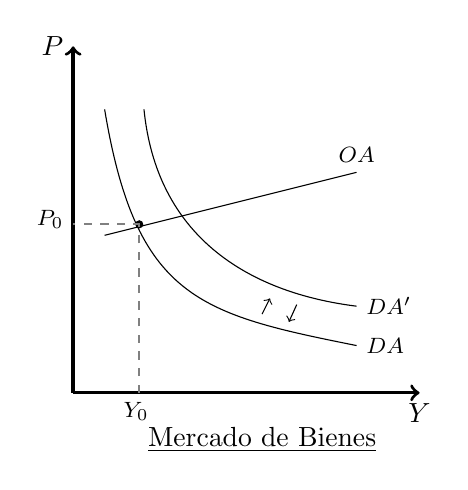
\begin{tikzpicture}[scale=0.4]
    \draw[very thick,<-] (0,11)--(0,0);
    \draw[very thick,->] (0,0)--(11,0) node[below]{$Y$};
    \node[left] at (0,11) {$P$};
    \node[] at(6,-1.5) {\underline{Mercado de Bienes}};
    \draw[thin] (1,9).. controls (2,3) and (4, 2.5) .. (9, 1.5) node [right]{\footnotesize $DA$};
    \draw[thin] (2.25,9).. controls (2.75,4) and (7, 3) .. (9, 2.75) node [right]{\footnotesize $DA'$};
    \draw[thin](1, 5)--(9,7) node [above]{\footnotesize $OA$};
    \draw[thin, ->] (6,2.5)--(6.25,3);
    \draw[thin, <-] (6.85,2.25)--(7.1,2.8);
    \node[below] at (2,0) {\footnotesize $Y_0$};
    \node[left] at (0,5.5) {\footnotesize $P_0$};
    \draw[fill] (2.1,5.35) circle [radius =0.11];
    \draw[thick, gray, dashed] (2.1,0)--(2.1,5.35)--(0,5.35);
    \end{tikzpicture}
    \end{center}
    \end{minipage}
    \begin{minipage}[b]{0.45\textwidth}
    \begin{center}
    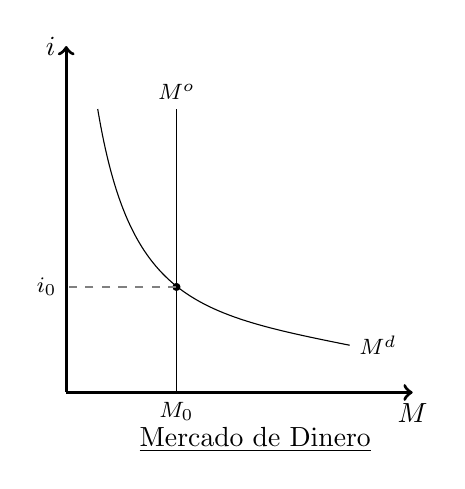
\begin{tikzpicture}[scale=0.4]
    \draw[very thick,<-] (0,11) node[left]{$i$}--(0,0);
    \draw[very thick,->] (0,0)--(11,0) node[below]{$M$};
    \node[right] at (0,11) {};
    \node[] at(6,-1.5) {\underline{Mercado de Dinero}};
    \draw[thin] (1,9).. controls (2,3) and (4, 2.5) .. (9, 1.5) node [right]{\footnotesize $M^{d}$};
    \draw[thin](3.5, 0)--(3.5, 9) node [above]{\footnotesize $M^{o}$};
    \node[below] at (3.5,0) {\footnotesize $M_0$};
    \node[left] at (0,3.35) {\footnotesize $i_0$};
    \draw[fill] (3.5,3.35) circle [radius =0.11];
    \draw[thick, gray, dashed] (3.5,3.35)--(0,3.35);
    \end{tikzpicture}
    \end{center}
    \end{minipage}
    \end{center}
    \end{figure}
    \end{center}
\end{frame}

\begin{frame}{Expansión fiscal con impuestos permanentes}
   Conclusiones:
   \begin{itemize}
       \item No hay efectos: lo que el gobierno gasta, la gente lo deja de gastar.
       \item La demanda agregada no se modifica
       \item No importa como es la curva de oferta
       \item Es decir el resultado es el mismo en el mundo clásico o keynesiano
   \end{itemize}
\end{frame}


\begin{frame}{Expansión fiscal c/ impuestos transitorios (clásico)}
    \begin{center}
        \begin{figure}[H]
        \renewcommand{\figurename}{Figure}
        \begin{center}
        \begin{minipage}[b]{0.45\textwidth}
        \begin{center}
        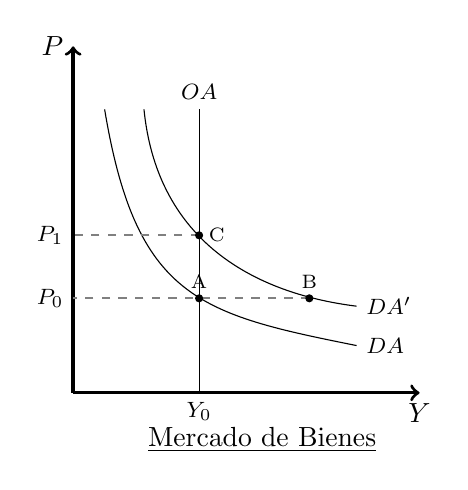
\begin{tikzpicture}[scale=0.4]
        \draw[very thick,<-] (0,11)--(0,0);
        \draw[very thick,->] (0,0)--(11,0) node[below]{$Y$};
        \node[left] at (0,11) {$P$};
        \node[] at(6,-1.5) {\underline{Mercado de Bienes}};
        \draw[thin] (1,9).. controls (2,3) and (4, 2.5) .. (9, 1.5) node [right]{\footnotesize $DA$};
        \draw[thin] (2.25,9).. controls (2.75,4) and (7, 3) .. (9, 2.75) node [right]{\footnotesize $DA'$};
        \draw[thin](4, 0)--(4, 9) node [above]{\footnotesize $OA$};
        \draw[thick, gray, dashed] (7.5,3)--(0,3);
        \draw[thick, gray, dashed] (4,5)--(0,5);
        \draw[fill] (7.5,3) circle [radius =0.11] node[above] {\scriptsize B};
        \draw[fill] (4,5) circle [radius =0.11] node[right] {\scriptsize C};
        \node[below] at (4,0) {\footnotesize $Y_0$};
        \node[left] at (0,3) {\footnotesize $P_0$};
        \node[left] at (0,5) {\footnotesize $P_1$};
        \draw[fill] (4,3) circle [radius =0.11] circle [radius =0.11] node[above] {\scriptsize A};
        \end{tikzpicture}
        \end{center}
        \end{minipage}
        \begin{minipage}[b]{0.45\textwidth}
        \begin{center}
        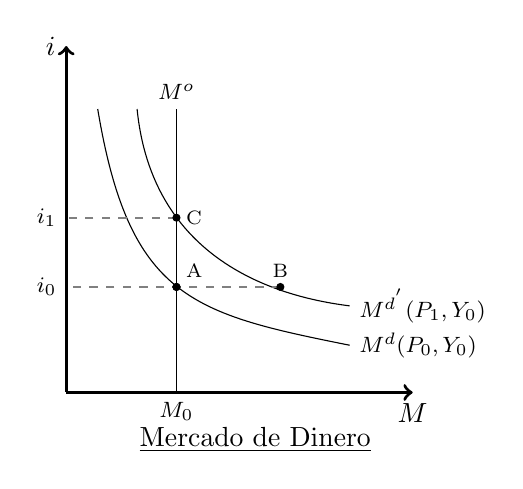
\begin{tikzpicture}[scale=0.4]
        \draw[very thick,<-] (0,11) node[left]{$i$}--(0,0);
        \draw[very thick,->] (0,0)--(11,0) node[below]{$M$};
        \node[right] at (0,11) {};
        \node[] at(6,-1.5) {\underline{Mercado de Dinero}};
        \draw[thin] (1,9).. controls (2,3) and (4, 2.5) .. (9, 1.5) node [right]{\footnotesize $M^{d} (P_0, Y_0)$};
        \draw[thin] (2.25,9).. controls (2.75,4) and (7, 3) .. (9, 2.75) node [right]{\footnotesize $M^{d^{'}} (P_1, Y_0)$};
        \draw[thin](3.5, 0)--(3.5, 9) node [above]{\footnotesize $M^{o}$};
        \draw[thick, gray, dashed] (6.8,3.35)--(0,3.35);
        \draw[thick, gray, dashed] (3.5,5.55)--(0,5.55);
        \draw[fill] (3.5,3.35) circle [radius =0.11] node[above right] {\scriptsize A};
        \draw[fill] (6.8,3.35) circle [radius =0.11] node[above] {\scriptsize B};
        \draw[fill] (3.5,5.55) circle [radius =0.11] node[right] {\scriptsize C};
        \node[below] at (3.5,0) {\footnotesize $M_0$};
        \node[left] at (0,3.35) {\footnotesize $i_0$};
        \node[left] at (0,5.55) {\footnotesize $i_1$};
        \draw[fill] (3.5,3.35) circle [radius =0.11];
        \end{tikzpicture}
        \end{center}
        \end{minipage}
        \end{center}
        \end{figure}
    \end{center} 
\end{frame}


\begin{frame}{Expansión fiscal c/impuestos transitorios (clásico)}
   
    \begin{itemize}
        \item La demanda agregada se expande porque la baja del consumo, a diferencia del caso anterior, no compensa plenamente el aumento del gasto público.
        \item En el mercado de bienes hay un exceso de demanda $\rightarrow$ los precios suben.
        \item El impacto en los precios aumenta la demanda de dinero.
        \item Por detrás, aumenta la tasa de interés en el mercado de crédito $\rightarrow$ disminuye la cantidad invertida.
        \item A la postre el crowding out es pleno.
        \item ¿Qué pasa cuando vuelven a bajar los impuestos?
        \begin{itemize}
            \item La demanda agregada cae y los precios también.
            \item Baja la tasa de interés.
            \item Volvemos al equilibrio \textbf{original}.
        \end{itemize}
    \end{itemize}
\end{frame}

\begin{frame}{Expansión fiscal c/impuestos transitorios (keynesiano)}
    \begin{center}
        \begin{figure}[H]
        \renewcommand{\figurename}{Figure}
        \begin{center}
        \begin{minipage}[b]{0.45\textwidth}
        \begin{center}
        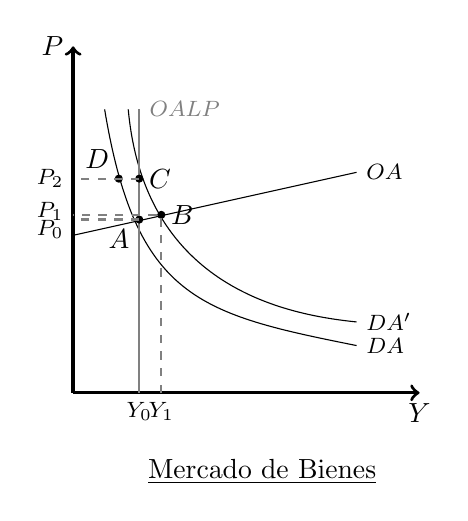
\begin{tikzpicture}[scale=0.4]
        \draw[very thick,<-] (0,11)--(0,0);
        \draw[very thick,->] (0,0)--(11,0) node[below]{$Y$};
        \node[left] at (0,11) {$P$};
        \node[] at(6,-2.5) {\underline{Mercado de Bienes}};
        \draw[thin] (1,9).. controls (2,3) and (4, 2.5) .. (9, 1.5) node [right]{\footnotesize $DA$};
        \draw[thin] (1.75,9).. controls (2.25,3.5) and (6.5,2.5) .. (9, 2.25) node [right]{\footnotesize $DA'$};
        \draw[thin] (0, 5)--(9, 7) node [right]{\footnotesize $OA$};
        \draw[thick, gray] (2.1,0)--(2.1,9) node [right]{\footnotesize $OALP$};
        \draw[fill] (2.1,5.5) circle [radius =0.11] node[below left] {$A$}; 
        \draw[fill] (2.8,5.65) circle [radius =0.11] node[right] {$B$}; 
        \draw[fill] (2.1,6.8) circle [radius =0.11] node[right] {$C$}; 
        \draw[fill] (1.45,6.8) circle [radius =0.11] node[above left] {$D$}; 
        \node[below] at (2.1,0) {\footnotesize $Y_0$};
        \node[below] at (2.8,0) {\footnotesize $Y_1$};
        \node[left] at (0,5.2) {\footnotesize $P_0$};
        \node[left] at (0,5.75) {\footnotesize $P_1$};
        \node[left] at (0,6.8) {\footnotesize $P_2$};
        \draw[thick, gray, dashed] (2.1,6.8)--(0,6.8);
        \draw[thick, gray, dashed] (2.8,0)--(2.8,5.65)--(0,5.65);
        \draw[thick, gray, dashed] (2.1,5.5)--(0,5.5);
        \end{tikzpicture}
        \end{center}
        \end{minipage}
        \begin{minipage}[b]{0.45\textwidth}
        \begin{center}
        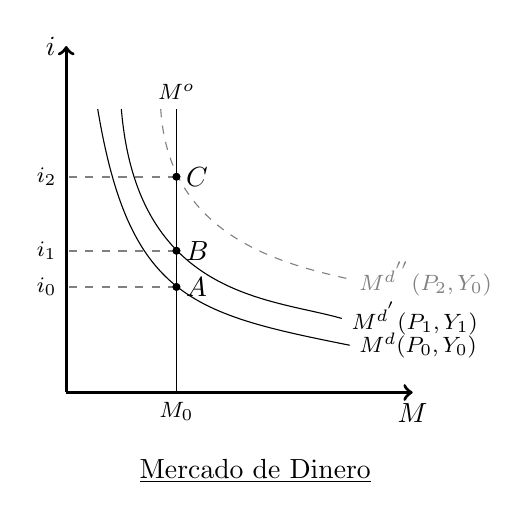
\begin{tikzpicture}[scale=0.4]
        \draw[very thick,<-] (0,11) node[left]{$i$}--(0,0);
        \draw[very thick,->] (0,0)--(11,0) node[below]{$M$};
        \node[right] at (0,11) {};
        \node[] at(6,-2.5) {\underline{Mercado de Dinero}};
        \draw[thin] (1,9).. controls (2,3) and (4, 2.5) .. (9, 1.5) node [right]{\footnotesize $M^{d} (P_0, Y_0)$};
        \draw[thin] (1.75,9).. controls (2.25,3) and (6.5, 3) .. (8.75, 2.35) node [right]{\footnotesize $M^{d^{'}} (P_1, Y_1)$};
        \draw[thin, gray, dashed] (3,9).. controls (3.25,5) and (6.75,4.1) .. (9,3.6) node [right]{\footnotesize $M^{d^{''}} (P_2, Y_0)$};
        \draw[thin](3.5, 0)--(3.5, 9) node [above]{\footnotesize $M^{o}$};
        \draw[thick, gray, dashed] (3.5,3.35)--(0,3.35);
        \draw[thick, gray, dashed] (3.5,4.5)--(0,4.5);
        \draw[thick, gray, dashed] (3.5,6.85)--(0,6.85);
        \draw[fill] (3.5,3.35) circle [radius =0.11] node[right] {$A$}; 
        \draw[fill] (3.5,4.5) circle [radius =0.11] node[right] {$B$}; 
        \draw[fill] (3.5,6.85) circle [radius =0.11] node[right] {$C$};
        \node[below] at (3.5,0) {\footnotesize $M_0$};
        \node[left] at (0,3.35) {\footnotesize $i_0$};
        \node[left] at (0,4.5) {\footnotesize $i_1$};
        \node[left] at (0,6.85) {\footnotesize $i_2$};
        \end{tikzpicture}
        \end{center}
        \end{minipage}
        \end{center}
        \end{figure}
    \end{center} 
\end{frame}

\begin{frame}{Expansión fiscal c/impuestos transitorios (keynesiano)}
   
\begin{itemize}
    \item La demanda agregada se expande porque la baja del consumo no compensa plenamente el aumento del gasto público.
    \item El exceso de demanda hace subir el producto y los precios $\rightarrow$ la demanda de dinero aumenta, empujando hacia arriba la tasa de interés.
    \item La tasa de interés sube menos (que en el caso clásico) y el producto se expande.
    \item Los precios empiezan a subir, nos movemos al equilibrio del punto $C$, que es identico al caso clásico.
    \item Cuando la politica se revierte, se pasa por una fase recesiva, porque la baja en la demanda agregada nos ubica en el punto D.
\end{itemize}
    
\end{frame}

\begin{frame}{¿Cómo funciona la política fiscal financiada con deuda?}
    \begin{itemize}
        \item Acá el punto clave es si los agentes anticipan la carga impositiva que implica la mayor deuda
        \begin{itemize}
            \item Si los agentes anticipan que el gobierno va a tener que subir impuestos en el futuro para pagar la deuda, entonces el efecto es el mismo que si se financiara con impuestos.
            \begin{itemize}
                \item En este caso decimos que los agentes son \textbf{ricardianos}.
            \end{itemize}
            \item Si los agentes no anticipan la carga impositiva, entonces el efecto es distinto.
            \begin{itemize}
                \item En este caso decimos que los agentes son \textbf{no ricardianos}.
            \end{itemize}
        \end{itemize}
        \item En la práctica se encuentra que el ahorro responde a la deuda, pero que la compensación no es plena.
        \item En tanto el efecto no es de compensación plena, hay un efecto expansivo en la demanda agregada (con efecto sobre el producto en un mundo keynesiano).
    \end{itemize}
\end{frame}

\begin{frame}{Ejemplo de equivalencia ricardiana}
    
    \begin{itemize}
        \item Supongamos dos periodos en los que el individuo tiene ingresos de 1000 y 1000
        \item El gobierno quiere gastar 100 y 100 
        \item Lo financia con deuda en el primer periodo y la tasa de interés es 10\%
        \item El agente enfrenta impuestos de 0 y 210
        \item Si consume su ingreso consumiría 1000 y 790 
        \item ¿Qué pasa si ahorra 100 en el primero período?
        \item Ahora puede consumir 900 y 900 (que es mejor que 1000 y 790)
        \item Pero 900 y 900 ¡es lo mismo que si el gobierno hubiera financiado los 100 con impuestos! 
    \end{itemize}
    
\end{frame}

\begin{frame}{¿Pero existe ese fenómeno Ricardiano? I}

    \begin{center}
        Correlación entre deuda pública y activos financieros netos acumulados por los hogares
    \end{center}

    \centering\includegraphics[width=11cm]{../Figures/C41.6.png}\  
\end{frame}

    
\begin{frame}{Política fiscal financiada con deuda y agentes ricardianos}
    
    \begin{itemize}
        \item Será otra vez relevante si el aumento es transitorio o permanente.
        \item Si el aumento del gasto público es permanente y se financia con deuda
        \begin{itemize}
            \item La gente se da cuenta de que en el futuro los impuestos tendrán que
            aumentar, y decidirán ahorrar más, anticipándose a lo que ocurrirá en
            el próximo período.
            \item En el mercado de crédito, el gobierno aumenta la
            demanda de crédito porque necesita crédito para financiarse, pero la
            gente ahorra más. El resultado es que la oferta de crédito aumenta en
            la misma magnitud que la demanda de crédito.
            \item El efecto se mantiene igual en el mundo keynesiano y clásico.
        \end{itemize}
        \item Si el aumento del gasto público es transitorio y financiado con deuda
        \begin{itemize}
            \item La demanda agregada se incrementa de la misma manera que cuando el aumento del gasto es transitorio, pero
            financiado a través de impuestos.
            \item Se produce la misma expansión en la demanda de crédito, pero es
            el gobierno quien lo causa, mientras que los individuos modifican muy
            poco su nivel de consumo.
        \end{itemize}
    \end{itemize}

\end{frame}

\begin{frame}{Política fiscal financiada con deuda y agentes ricardianos (permanente)}
   
    \begin{center}
        \begin{figure}[H]
        \renewcommand{\figurename}{Figure}
        \begin{center}
        \begin{minipage}[b]{0.45\textwidth}
        \begin{center}
        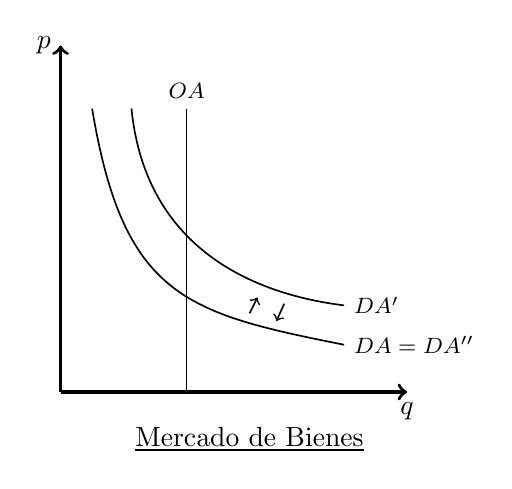
\begin{tikzpicture}[scale=0.4]
        \draw[very thick,<-] (0,11)--(0,0);
        \draw[very thick,->] (0,0)--(11,0) node[below]{$q$};
        \node[left] at (0,11) {$p$};
        \node[] at(6,-1.5) {\underline{Mercado de Bienes}};
        \draw[semithick] (1,9).. controls (2,3) and (4, 2.5) .. (9, 1.5) node [right]{\footnotesize $DA=DA''$};
        \draw[semithick] (2.25,9).. controls (2.75,4) and (7, 3) .. (9, 2.75) node [right]{\footnotesize $DA'$};
        \draw[semithick](4, 0)--(4, 9) node [above]{\footnotesize $OA$};
        \draw[semithick, ->] (6,2.5)--(6.25,3);
        \draw[semithick, <-] (6.85,2.25)--(7.1,2.8);
        \end{tikzpicture}
        \end{center}
        \end{minipage}
        \begin{minipage}[b]{0.45\textwidth}
        \begin{center}
        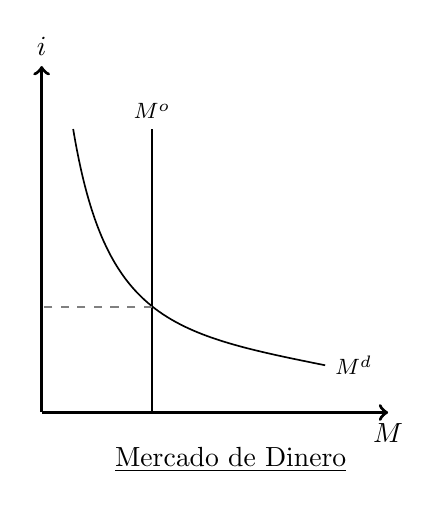
\begin{tikzpicture}[scale=0.4]
        \draw[very thick,<-] (0,11) node[above]{$i$}--(0,0);
        \draw[very thick,->] (0,0)--(11,0) node[below]{$M$};
        \node[right] at (0,11) {};
        \node[] at(6,-1.5) {\underline{Mercado de Dinero}};
        \draw[semithick] (1,9).. controls (2,3) and (4, 2.5) .. (9, 1.5) node [right]{\footnotesize $M^{d}$};
        \draw[semithick](3.5, 0)--(3.5, 9) node [above]{\footnotesize $M^{o}$};
        \draw[thick, gray, dashed] (3.5,3.35)--(0,3.35);
        \end{tikzpicture}
        \end{center}
        \end{minipage}
        \end{center}
        \end{figure}
    \end{center}
\end{frame}

\begin{frame}{Política fiscal financiada con deuda y agentes no ricardianos}
    \begin{itemize}
        \item Ahora los agentes no internalizan que la deuda pública implica impuestos futuros.
        \item Si esto es así, el consumo no disminuye y la demanda agregada se expande ante un aumento en el gasto público.
        \item Como esto sucede para cualquier tipo de gasto público, ya no es relevante si es transitorio o permanente.
        \item En el caso clásico, el efecto sobre el producto es nulo $\rightarrow$ el efecto es sobre los precios y la tasa de interés $\rightarrow$ otra vez \textit{crowding out} del gasto sobre el consumo y la inversion.
        \item Para el caso keynesiano, será relevante el concepto de \textbf{multiplicador}.
    \end{itemize}
\end{frame}

\begin{frame}{Política fiscal financiada con deuda y agentes no ricardianos (clásicos)}
    \begin{center}
        \begin{figure}[H]
        \renewcommand{\figurename}{Figure}
        \begin{center}
        \begin{minipage}[b]{0.45\textwidth}
        \begin{center}
        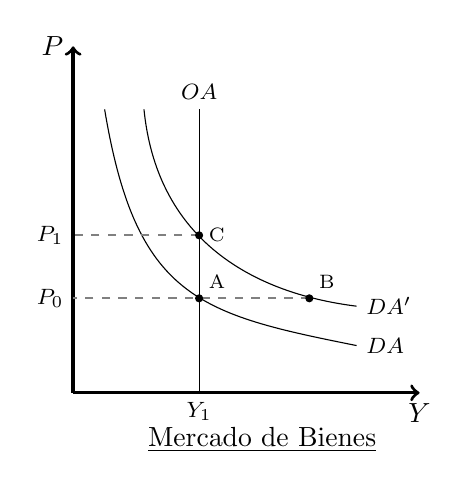
\begin{tikzpicture}[scale=0.4]
        \draw[very thick,<-] (0,11)--(0,0);
        \draw[very thick,->] (0,0)--(11,0) node[below]{$Y$};
        \node[left] at (0,11) {$P$};
        \node[] at(6,-1.5) {\underline{Mercado de Bienes}};
        \draw[thin] (1,9).. controls (2,3) and (4, 2.5) .. (9, 1.5) node [right]{\footnotesize $DA$};
        \draw[thin] (2.25,9).. controls (2.75,4) and (7, 3) .. (9, 2.75) node [right]{\footnotesize $DA'$};
        \draw[thin](4, 0)--(4, 9) node [above]{\footnotesize $OA$};
        \draw[thick, gray, dashed] (7.5,3)--(0,3);
        \draw[thick, gray, dashed] (4,5)--(0,5);
        \draw[fill] (4,3) circle [radius =0.11] node[above right] {\scriptsize A};
        \draw[fill] (7.5,3) circle [radius =0.11] node[above right] {\scriptsize B};
        \draw[fill] (4,5) circle [radius =0.11] node[right] {\scriptsize C};
        \node[below] at (4,0) {\footnotesize $Y_1$};
        \node[left] at (0,3) {\footnotesize $P_0$};
        \node[left] at (0,5) {\footnotesize $P_1$};
        \end{tikzpicture}
        \end{center}
        \end{minipage}
        \begin{minipage}[b]{0.45\textwidth}
        \begin{center}
        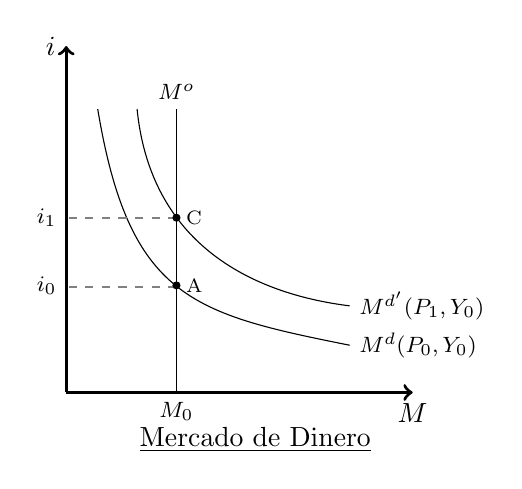
\begin{tikzpicture}[scale=0.4]
        \draw[very thick,<-] (0,11) node[left]{$i$}--(0,0);
        \draw[very thick,->] (0,0)--(11,0) node[below]{$M$};
        \node[right] at (0,11) {};
        \node[] at(6,-1.5) {\underline{Mercado de Dinero}};
        \draw[thin] (1,9).. controls (2,3) and (4, 2.5) .. (9, 1.5) node [right]{\footnotesize $M^{d} (P_0, Y_0)$};;
        \draw[thin] (2.25,9).. controls (2.75,4) and (7, 3) .. (9, 2.75) node [right]{\footnotesize $M^{d'} (P_1, Y_0)$};
        \draw[thin](3.5, 0)--(3.5, 9) node [above]{\footnotesize $M^{o}$};
        \draw[thick, gray, dashed] (3.5,3.35)--(0,3.35);
        \draw[thick, gray, dashed] (3.5,5.55)--(0,5.55);
        \draw[fill] (3.5,3.4) circle [radius =0.11] node[right] {\scriptsize A}; 
        \draw[fill] (3.5,5.55) circle [radius =0.11] node[right] {\scriptsize C};  
        \node[below] at (3.5,0) {\footnotesize $M_0$};
        \node[left] at (0,3.4) {\footnotesize $i_0$};
        \node[left] at (0,5.55) {\footnotesize $i_1$};
        \end{tikzpicture}
        \end{center}
        \end{minipage}
        \end{center}
        \end{figure}
    \end{center} 
\end{frame}

\begin{frame}{Política fiscal financiada con deuda y agentes no ricardianos (keynesiano)}
    \begin{center}
        \begin{figure}[H]
        \renewcommand{\figurename}{Figure}
        \begin{center}
        \begin{minipage}[b]{0.45\textwidth}
        \begin{center}
        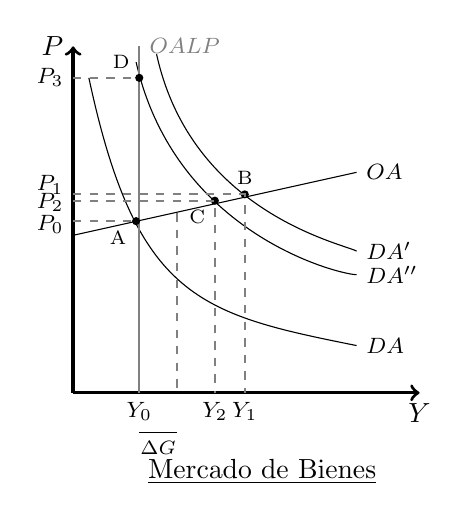
\begin{tikzpicture}[scale=0.4]
        \draw[very thick,<-] (0,11)--(0,0);
        \draw[very thick,->] (0,0)--(11,0) node[below]{$Y$};
        \node[left] at (0,11) {$P$};
        \node[] at(6,-2.5) {\underline{Mercado de Bienes}};
        \draw[thin] (0.5,10).. controls (2,3) and (4, 2.5) .. (9, 1.5) node [right]{\footnotesize $DA$};
        \draw[thin] (2.65,10.75).. controls (3.75,5.75) and (8.5, 4.75) .. (9, 4.5) node [right]{\footnotesize $DA'$};
        \draw[thin] (2,10.5).. controls (3.25,5) and (8.5, 3.75) .. (9, 3.75) node [right]{\footnotesize $DA''$};
        \draw[thin](0, 5)--(9, 7) node [right]{\footnotesize $OA$};
        \draw [thin](2.1,-1.25) -- (3.3,-1.25);
        \draw (2.7,-1.75) node[]{\scriptsize $\Delta G $};
        \draw[thick, gray] (2.1,0)--(2.1,11) node [right]{\footnotesize $OALP$};
        \draw[thick, gray, dashed] (3.3,5.7)--(3.3,0); 
        \draw[fill] (2,5.45) circle [radius =0.11] node[below left] {\scriptsize A};  
        \draw[fill] (5.45,6.3) circle [radius =0.11] node[above] {\scriptsize B}; 
        \draw[fill] (4.5,6.1) circle [radius =0.11] node[below left] {\scriptsize C};  
        \draw[fill] (2.1,10) circle [radius =0.11] node[above left] {\scriptsize D};  
        \node[below] at (2.1,0) {\footnotesize $Y_0$};
        \node[below] at (5.45,0) {\footnotesize $Y_1$};
        \node[below] at (4.5,0) {\footnotesize $Y_2$};
        \node[left] at (0,5.35) {\footnotesize $P_0$};
        \node[left] at (0,6.6) {\footnotesize $P_1$};
        \node[left] at (0,6.05) {\footnotesize $P_2$};
        \node[left] at (0,10) {\footnotesize $P_3$};
        \draw[thick, gray, dashed] (0,5.45)--(2,5.45);
        \draw[thick, gray, dashed] (0,6.3)--(5.45,6.3)--(5.45,0);
        \draw[thick, gray, dashed] (0,6.1)--(4.5,6.1)--(4.5,0);
        \draw[thick, gray, dashed] (0,10)--(2.1,10);
        \end{tikzpicture}
        \end{center}
        \end{minipage}
        \begin{minipage}[b]{0.45\textwidth}
        \begin{center}
        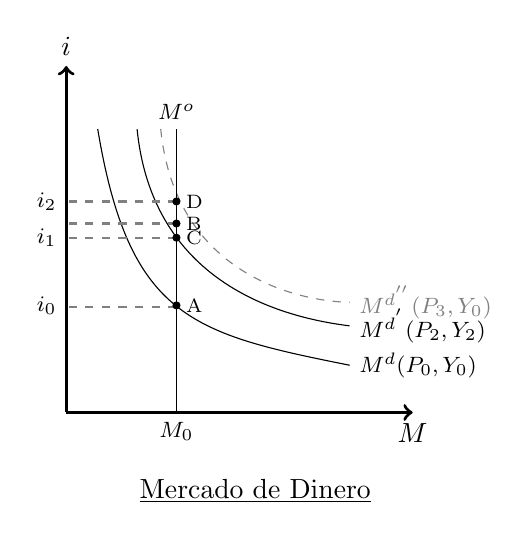
\begin{tikzpicture}[scale=0.4]
        \draw[very thick,<-] (0,11) node[above]{$i$}--(0,0);
        \draw[very thick,->] (0,0)--(11,0) node[below]{$M$};
        \node[right] at (0,11) {};
        \node[] at(6,-2.5) {\underline{Mercado de Dinero}};
        \draw[thin] (1,9).. controls (2,3) and (4, 2.5) .. (9, 1.5) node [right]{\footnotesize $M^{d} (P_0, Y_0)$};
        \draw[thin] (2.25,9).. controls (2.75,4) and (7, 3) .. (9, 2.75) node [right]{\footnotesize $M^{d^{'}} (P_2, Y_2)$};
        \draw[thin, gray, dashed] (3,9).. controls (3.5,4) and (8, 3.5) .. (9,3.5) node [right]{\footnotesize $M^{d^{''}} (P_3, Y_0)$};
        \draw[thin](3.5, 0)--(3.5, 9) node [above]{\footnotesize $M^{o}$};
        \draw[thick, gray, dashed] (3.5,3.35)--(0,3.35);
        \draw[thick, gray, dashed] (3.5,5.55)--(0,5.55);
        \draw[thick, gray, dashed] (3.5,6)--(0,6);
        \draw[thick, gray, dashed] (3.5,6.7)--(0,6.7);
        \draw[fill] (3.5,3.4) circle [radius =0.11] node[right] {\scriptsize A};
        \draw[fill] (3.5,5.55) circle [radius =0.11] node[right] {\scriptsize C};  
        \draw[fill] (3.5,6) circle [radius =0.11] node[right] {\scriptsize B};  
        \draw[fill] (3.5,6.7) circle [radius =0.11] node[right] {\scriptsize D}; 
        \node[below] at (3.5,0) {\footnotesize $M_0$};
        \node[left] at (0,3.4) {\footnotesize $i_0$};
        \node[left] at (0,5.55) {\footnotesize $i_1$};
        \node[left] at (0,6.7) {\footnotesize $i_2$};
        \end{tikzpicture}
        \end{center}
        \end{minipage}
        \end{center}
        \end{figure}
    \end{center}
\end{frame}


\begin{frame}{Política fiscal financiada con deuda y agentes no ricardianos (keynesiano)}
   
    \begin{itemize}
        \item El aumento en la demanda agregada incrementa el producto en una proporción mayor que la expansión en el gasto público, debido al efecto \textbf{multiplicador}.
        \item La expansión del producto va a producir un aumento en la demanda de dinero que, a su vez, elevará la tasa de interés, contrayendo algo la demanda agregada.
        \item Si bien sube la tasa de interés, el efecto del multiplicador prima por ende hay expansión en el producto.
        \item En el largo plazo, los precios tienden al alza.
    \end{itemize}
\end{frame}


\begin{frame}{Discusión}

    \begin{itemize}
    \item Para un clásico hay poco por hacer: más vale concentrarte en lo estructural (competencia, apertura, instituciones).
    \item En el mundo keynesiano, al menos hay margen, pero…
    \item A) La mayor parte de los cambios en el producto son generados por cambios en C e I, causados por los agentes individuales, inducidos por el ambiente político y las expectativas
    \item B) ¿Estamos seguros el gobierno será efectivo o incluso si actuará cuando debe actuar? 
    \end{itemize}

\end{frame}

\begin{frame}{Caveats a la política macroeconómica}
    \begin{itemize}
    \item Puede existir un problema de rezagos: las políticas pueden hacerse en un momento inadecuado
    \item Podes pensar que podes cuando no podes (si el mundo es clásico, las políticas sólo van a resultar en inflación o deflación)
    \item Si el marco político genera gobiernos débiles, puede existir prociclicalidad fiscal o exceso de gasto
    \item Las políticas pueden incrementar la incertidumbre y las expectativas son \textbf{fundamentales}.
    \item La gente puede anticipar estas políticas haciéndolas menos efectivas (inconsistencia temporal y expectativas racionales), por ejemplo si vos aumentas el dinero y la gente se da cuenta al toque, los precios suben y no lográs nada
    \end{itemize}
\end{frame}

\end{document}







